\documentclass[a4paper]{jpconf}
\usepackage{graphicx}
\usepackage[english]{babel}
\usepackage{amsmath}
\usepackage{amsfonts}
\usepackage{amssymb}


\begin{document}
\title{High performance computing for global optimization problems}


\author{K.A. Barkalov, V.P. Gergel}

\address{Lobachevsky State University of Nizhni Novgorod, Gagarin avenue 23, 
Nizhnш Novgorod, Russia, 603950}

\ead{konstantin.barkalov@itmm.unn.ru}


\begin{abstract}
In the present work, the multiextremal optimization problems and a high-
performance parallel algorithm for solving these ones are considered. The 
investigation of the algorithm scalability has been carried out on the 
problem class, in which the computation costs of the function value evaluations can be varied at different iteration points. The algorithm proposed in the present work can utilize 
the CPUs (for solving more complex subproblems) as well as the GPUs (for 
solving the simple subproblems). The results of numerical experiments 
demonstrating the speedup when solving a series of multiextremal constrained 
problems are presented.
\end{abstract}

\section{Introduction}
In the present paper, the constrained multiextremal optimization problems and 
the parallel methods for solving these ones are considered. The fact that the 
global extremum is an integral characteristic of a problem is an important 
feature of the multiextremal problems. Thus, its finding is related to the 
construction of a coverage of the search domain and the computing the 
 function values at all points of this coverage. The dimensionality 
affects the difficulty of solving the problems of considered class crucially: 
the computational costs grow with increasing this one exponentially, 
therefore, for solving such problems, the methods are required, which 
generate a nonuniform grid in the search domain, denser near the 
global minimizer and more sparse far away from this one. In the 
present paper, the results of scalability investigation of the parallel 
index global optimization algorithm developed in Lobachevsky State 
University of Nizhni Novgorod \cite{Strongin2000,Strongin2013} and implemented in the Globalizer 
system \cite{Globalizer,Globalizer1} are presented.

Within the framework of the discussed approach, the solving of the 
multidimensional problems is reduced to the solving of a set of the connected 
subproblems of less dimensionality. The corresponding dimensionality 
reduction is based on the use of the evolvents of a unit interval on the real 
axis onto a hypercube. The continuous unambiguous mappings like Peano curves, 
called also the space-filling curves, play the role of such evolvents. 
The nested optimization scheme is one more mechanism used for reducing the 
dimensionality of the problem being solved. The numerical methods allowing 
the efficient utilization of such reduction schemes had been developed 
in details and substantiated in \cite{Strongin2000,Strongin2013}.

In the algorithms considered in the present paper the objective function and constraints are assumed to be Lipschitzian that is typical for many other approaches to the development of the parallel optimization algorithms (see, for example, \cite{Jones,Zilinskas,Evtushenko2009,Evtushenko2014}). This assumption is natural for many applied problems since the relative variations of the functions generally cannot exceed a certain threshold determined by the bounded energy of changes occurring in the system under study. Also, a standard assumption is that the execution of a single trial (the computing of the values of the objective function and constraints at a point in the search domain) is a time-consuming operation since it 
utilized the results of numerical modeling. 

An assumption on different costs of computing the problem functions subject to 
various components of the vector of parameters is a novel element investigated in the present work. 
It is assumed that it is possible to select the ``difficult'' and ``easy'' parts 
of the functions connected with each other. An example of a problem of this type has been considered in \cite{Strongin2017}.
Then, the solving of the ``difficult'' part of the problem (for which the execution of time-consuming algorithms is required to conduct the trials) can be performed on CPU using an efficient index global optimization algorithm. The ``easy'' part of the problem (the execution of which doesn't require the complex algorithms 
and can be transferred to an accelerator easily) can be solved on GPU using 
the uniform grid technique. Obviously, in this case a major portion of the trials 
will be carried out on GPU, and the minor one will be carried out on CPU. However, 
because of the difference in the difficulties of the subproblems solved on 
different units, a speedup of the algorithm as a whole can be expected. 
The proposed approach has been implemented in Globalizer parallel software 
system for solving the global optimization problem developed in Lobachevsky 
State University of Nizhni Novgorod. 

\section{Problem statement}

Let us consider the $N$-dimensional global optimization problem
\begin{equation}\label{problem}
\varphi(y^\ast)=\min{\left\{\varphi(y): y \in D, \; g_i(y)\leq 0, \; 1 \leq i 
\leq m\right\}}
\end{equation}
with the search domain
\[
D=\left\{y\in R^N: a_j\leq y_j \leq b_j, 1\leq j \leq N \right\}.
%D=\left\{y\in R^N: a_i\leq y_i \leq b_i, 1\leq i \leq N\right\}.
\]

The objective function $\varphi(y)$ (henceforth denoted by $g_{m+1}(y)$) and
the left-hand sides $g_i(y), \; 1\leq i \leq m$, of the constraints
satisfy the Lipschitz conditions with constants $L_i$, $1 \leq i \leq
m+1$, respectively, and may be multiextremal. It is assumed that the
functions $g_i(y),\; 1 \leq i \leq m+1$, are defined and computable only in 
the corresponding domains
\[
Q_1=D, \; Q_{i+1}=\left\{y \in Q_i : g_i(y) \leq 0 \right\}, \; 1 \leq i \leq 
m.
\]

These conditions allow for the introduction of a classification of the
points $y \in D$ according to the number $\nu (y)$ of the constraints
computed at this point. 

Thus, a \textit{trial} at a point $y^k \in D$ executed at the $k$-th
iteration of the algorithm will consist in computing the values 
$g_1(y^k),...,g_\nu(y^k),$ where the
index $\nu \leq m$ is determined by the conditions
\[
	g_i(y^k )\leq 0, \; 1 \leq i < \nu, \; g_\nu(y^k)>0, \; \nu \leq m.
\]
The occurrence of the first violation of the constraint terminates the
trial. In the case when the point $y^k$ is a feasible one, i.e. when
$y \in Q_{m+1}$, the trial includes the computation of the values of
all the functions of the problems and the index is assumed to be
$\nu=m+1$. The pair of values
\[
\nu=\nu(y^k), \; z^k=g_\nu(y^k)
\]
is a \textit{trial result}.

The main idea of the index algorithm which can be applied to solving such problems 
with partially defined functions consists in the reduction of the initial multidimensional problem to a set of 
the subproblems of less dimensionality and the solving of these ones 
in parallel. The index method and dimensionality reduction schemes are described briefly in the next sections.


\section{Parallel index method}

In this section we consider a one-dimensional multiextremal optimization problem
\[
\varphi(x^\ast)=\min{\left\{\varphi(x): x \in [a,b], \; g_i(x)\leq 0, \; 1 \leq i \leq m\right\}}.
\]
Let us describe a rules of parallel index method for the case when the algorithm carries out during one iteration $p>1$ trials simultaneously (each trial in a separate thread or process). Let $k(n)$ be the total number of trials, carried out after $n$ parallel iterations.

Suppose $n\geq 1$  iterations of the method have been carried out, in which trials were performed at $k=k(n)$ points $x^i,1\leq i \leq k$. Then points $x^{k+1},\dots,x^{k+p}$  of search trials of the next $n+1$ iteration are determined according to the following rules.

Rule 1. Renumber the points $x^1,...,x^k$ of the preceding trials by the
lower indices in ascending order of coordinate values, i.e.
\[
0=x_0<x_1<\dots <x_k<x_{k+1}=1,
\]
and juxtapose to them the values $z_i=g_\nu(x_i), \; \nu=\nu(x_i), \; 1
\leq i \leq k$, computed at these points. The points $x_0=0$ and
$x_{k+1}=1$ are introduced additionally, while the values $z_0$ and
$z_{k+1}$ are not defined.

Rule 2. Classify the indices $i, \; 1 \leq i \leq k$, of the trial points
according to the number of the problem constraints fulfilled at these
points, by constructing the sets
\[
I_\nu =\left\{i:1 \leq i \leq k, \; \nu=\nu(x_i) \right\}, \; 1 \leq \nu \leq m+1,
\]
containing the numbers of all the points $x_i, \; 1 \leq i \leq k$, with
the same values of $\nu$. The end points $x_0=0$ and $x_{k+1}=1$ are
interpreted as the ones having indices equal to zero. An additional set,
$I_0=\left\{0,k+1\right\}$, corresponds to them.

Determine the maximum value of the index:
\[
M=\max\left\{\nu(x_i), \; 1 \leq i \leq k \right \}.
\]

Rule 3. Compute the current lower estimates
\begin{equation}\label{Rule_Mu}
\mu_\nu = \max\left\{ \frac{\left|z_i-z_j\right|}{ x_i - x_j }, \; i,j \in I_\nu, \; i>j \right\}, \; 1 \leq \nu \leq m+1,
\end{equation}
for the unknown Lipschitz constants $L_\nu$ of the functions $g_\nu(x),1
\leq \nu \leq m+1$. If a set $I_\nu$ contains less than two elements, or
if $\mu_\nu$ is equal to zero, then assume $\mu_\nu=1$.

Rule 4. For all nonempty sets $I_\nu, \; 1 \leq \nu \leq m+1$, compute the
estimates
\[
z_\nu^\ast = \left\{
   \begin{array}{lr}
     -\epsilon_\nu, & \nu < M,\\
     \min\{ g_\nu(x_i): i\in I_\nu \}, & \nu = M,
   \end{array}
\right.
 \]
where the nonnegative numbers $(\epsilon_1,...,\epsilon_m)$ are parameters
of the algorithm.

Rule 5. For each interval ($x_{i-1},x_i), \; 1 \leq i \leq k+1,$ compute
the \textit{characteristics} $R(i)$ :
\[
R(i)=2\Delta_i-4\frac{z_i-z_\nu^\ast}{r_\nu \mu_\nu}, \; \nu=\nu(x_i)>\nu(x_{i-1}),
\]
\begin{equation}\label{Rule_R}
R(i)=\Delta_i+\frac{(z_i-z_{i-1})^2}{r_\nu^2 \mu_\nu^2\Delta_i}-2\frac{z_i+z_{i-1}-2z_\nu^\ast}{r_\nu \mu_\nu}, \;  \nu=\nu(x_i)=\nu(x_{i-1}),
\end{equation}
\[
R(i)=2\Delta_i-4\frac{z_{i-1}-z_\nu^\ast}{r_\nu \mu_\nu}, \; \nu=\nu(x_{i-1})>\nu(x_i),
\]
where $\Delta_i=x_i - x_{i-1}$. The values $r_\nu > 1, \; 1 \leq
\nu \leq m+1,$ are parameters of the algorithm. An appropriate selection
of $r_\nu$ allows to consider the product $r_\nu \mu_\nu$ as an estimate
of the Lipschitz constants $L_\nu, \; 1 \leq \nu \leq m+1$.

Rule 6. Arrange characteristics  $R(i), 1 \leq i \leq k+1$, in decreasing order 
\begin{equation}\label{Rule_Max}
R(t_1)\geq R(t_2)\geq \dots \geq R(t_{k}) \geq R(t_{k+1})
\end{equation}
and select $p$ maximum characteristics with interval numbers $t_j, 1\leq j \leq p$.

Rule 7. Carry out new trials at points $x^{k+j}\in(x_{t_j-1},x_{t_j}), 1\leq j\leq p$, calculated using the formulae
\[
x^{k+j} = \frac{x_{t_j} + x_{t_j-1}}{2}, \textrm{ if } \nu(x_{t{_j}-1}) \neq \nu(x_{t_j}),
\]
\begin{equation}\label{Rule_X}
x^{k+j} = \frac{x_{t_j}+x_{t_j-1}}{2} - \frac{z_{t_j}-z_{t_j-1}}{2r_\nu \mu_\nu}, \textrm{ if } \nu=\nu(x_{t_j-1})=\nu(x_{t_j}).
\end{equation}

The algorithm terminates if the condition $\Delta_{t_j}<\epsilon$ is satisfied at least for one number $t_j, 1 \leq j \leq p$ ; $\epsilon>0$ is the predefined accuracy.

This method of parallelization has the following justification. The characteristics of intervals (\ref{Rule_R}) used in the index method can be considered as probability measures of the global minimum point location in these intervals. Inequalities (\ref{Rule_Max}) arrange intervals according to their characteristics, and trials are carried out in parallel in the first $p$ intervals with the largest probabilities.

\section{Dimensionality reduction}

\subsection{Dimensionality reduction using space-filling curves}

The use of Peano curve $y(x)$ 
\[
\left\{y\in R^N: -2^{-1}\leq y_i \leq 2^{-1}, 1 \leq i \leq 
N\right\}=\left\{y(x):0\leq x \leq 1 \right\}
\]
unambiguously mapping the interval of real axis $[0,1]$ onto a $N$-dimensional cube is the first of the dimensionality reduction methods considered.  To implement this method of dimensionality reduction a 
numerically constructed curve (\textit{evolvent}) is used. The evolvent is 
$2^{-m}$ accurate approximation of the theoretical Peano curve in $L_\infty$ 
metric, where $m$ is an evolvent construction parameter. Problems of 
numerical construction of the evolvents and the corresponding theory are 
considered in detail in \cite{Strongin2000}. Examples of the evolvent with different $m$ in two dimensions are given in figure~\ref{fig:0}.


\begin{figure}[t]
\begin{minipage}{0.32\linewidth}
\center{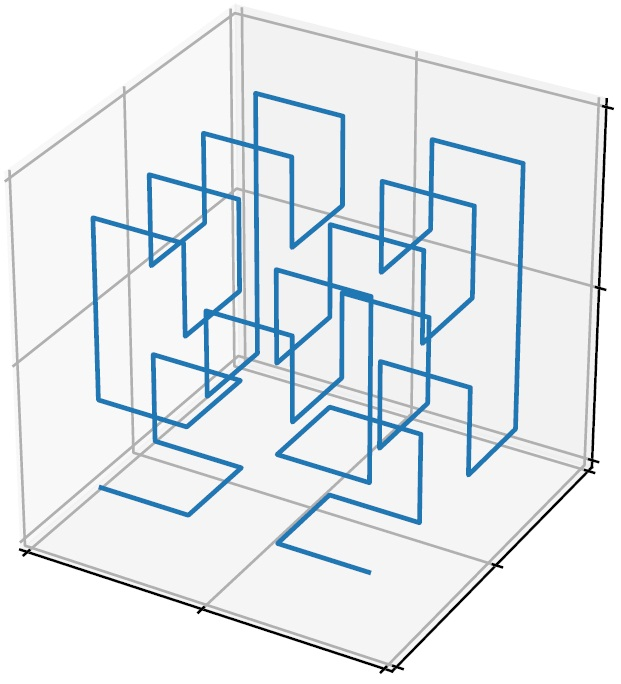
\includegraphics[width=1.0\linewidth]{fig1a.JPG} \\ (a)}
\end{minipage}
%\hfill
\begin{minipage}{0.32\linewidth}
\center{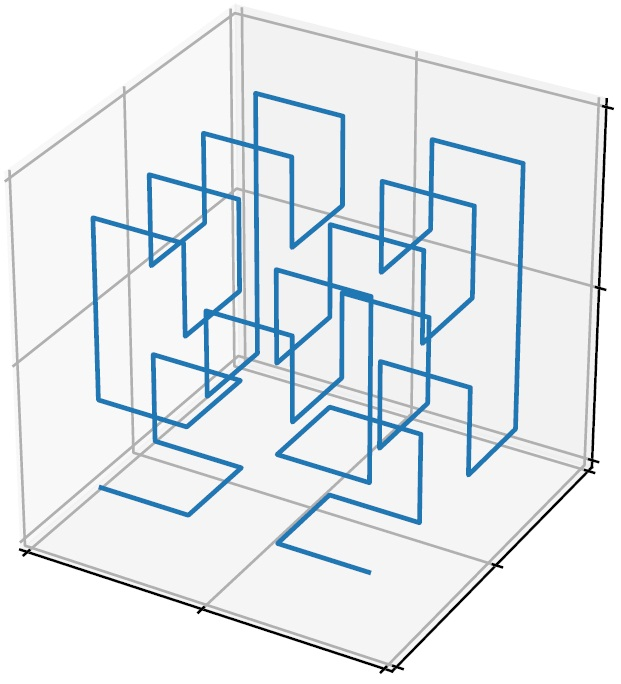
\includegraphics[width=1.0\linewidth]{fig1b.JPG} \\ (b)}
\end{minipage}
\begin{minipage}{0.32\linewidth}
\center{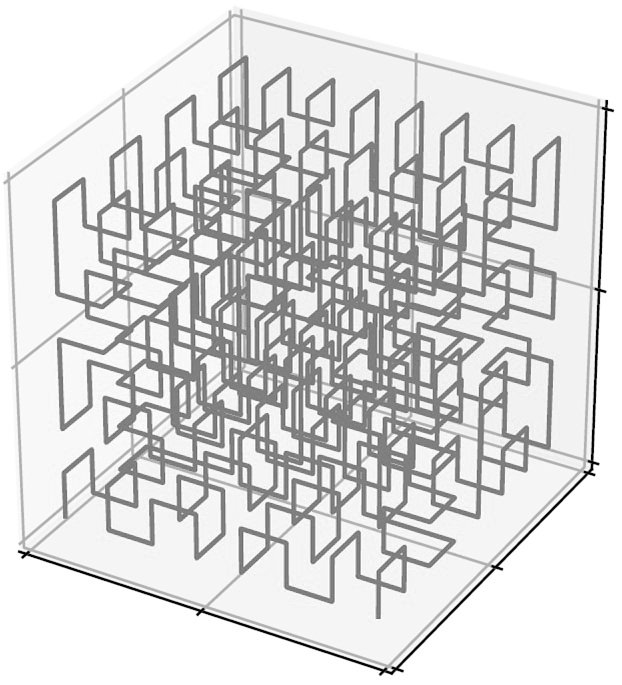
\includegraphics[width=1.0\linewidth]{fig1c.JPG} \\ (c)}
\end{minipage}
\caption{Evolvents in two dimensions with (a) $m=3$, (b) $m=4$ and (c) $m=5$}
\label{fig:0}
\end{figure}



By using this kind of mapping it is possible to reduce the multidimensional 
problem~(\ref{problem}) to a univariate problem
\[
\varphi(y(x^\ast))=\min \left\{\varphi(y(x)): x \in [0,1], \; g_i(y(x))\leq 
0, \; 1 \leq i \leq m\right\}.
\]

The considered dimensionality reduction scheme juxtaposes a
multidimensional problem with lipschitzian functions to a univariate
problem where the corresponding functions satisfy the uniform H{\"o}lder
condition (see \cite{Strongin2000}), i.e.
\begin{equation}\label{holder}
\left|g_i(y(x'))-g_i (y(x''))\right| \leq H_i \left|x'-x'' \right|^{1/N}, \; 
x',x''\in [0,1], \; 1\leq i \leq m+1.
\end{equation}
Here $N$ is the dimensionality of the initial multidimensional problem and
the coefficients $H_i$ are related with the Lipschitz constants $L_i$ of
the initial problem by the inequalities $H_i \leq 2L_i \sqrt{N+3}$.

Relation (\ref{holder}) allows modification of the parallel index algorithm described in previous section for solving multidimensional problems reduced to one-dimensional ones. For this purpose the intervals lengths $\Delta_i$ from the rules (\ref{Rule_Mu}) and (\ref{Rule_R}) of the index method are replaced with the lengths in a new metric
\[
\Delta_i = \left(x_i-x_{i-1}\right)^{1/N},
\]
and formula (\ref{Rule_X}) is replaced by the expression
\[
x^{k+j} = \frac{x_{t_j}+x_{t_j-1}}{2} - \frac{\mathrm{sign}(z_{t_j}-z_{t_j-1})}{2r_\nu}\left[\frac{\left|z_{t_j}-z_{t_j-1}\right|}{\mu_\nu}\right]^N, \; \nu=\nu(x_{t_j-1})=\nu(x_{t_j}).
\]

Various modifications of this algorithm and the corresponding theory of convergence are given in \cite{Strongin2000,Strongin2013,Gergel2005}.


\subsection{Nested optimization scheme}

Nested optimization scheme is based on relation (see \cite{Strongin2013})
\[
\min_{y \in D}{\left\{\varphi(y): \; g_i(y)\leq 0, \; 1 \leq i \leq 
m\right\}}= \min_{u_1\in D_1}\min_{u_2\in D_2}...\min_{u_M\in D_M 
}{\left\{\varphi(y): \; g_i(y)\leq 0, \; 1 \leq i \leq m\right\}},
\]
which allows replacing the solving of multidimensional problem 
(\ref{problem}) by solving a family of subproblems related to each other 
recursively.
Here we consider vector $y$ as a vector of block variables
\[
y=(y_1,y_2,...,y_N)=(u_1,u_2,...,u_M),
\]
where the $i$-th block variable $u_i$ is a vector of $N_i$ components of 
vector $y$, taken serially, i.e. $u_1=(y_1,y_2,...,y_{N_1})$, 
$u_2=(y_{N_1+1},y_{N_1+2},...,y_{N_1+N_2})$,..., $u_M=(y_{N-N_M+1},y_{N-
N_M+2},...,y_{N})$, and $N_1+N_2+...+N_M=N$. 
The subdomains $D_i, 1 \leq i \leq M$, are projections of initial search 
domain $D$ onto the subspaces corresponding to the variables $u_i, 1 \leq i 
\leq M$.

The number of vectors $M$ and the quantity of components in each vector $N_1, N_2,...,N_M$ are the parameters of the nested optimization scheme and can be used to form the subproblems with necessary properties. For example, if  $M=N$ i.e. $u_i=y_i, 1\leq i \leq N,$ each nested subproblem is a one-dimensional one. If $M=1$, i.e. $u=u_1=y$ , the solving of the problem is equivalent to solving this one using a single evolvent mapping $[0,1]$ into $D$; the nested subproblems are absent. 

In the present study, this scheme has been applied for $M=2$
\[
\min_{y \in D}{\left\{\varphi(y): \; g_i(y)\leq 0, \; 1 \leq i \leq 
m\right\}}= \min_{u_1\in D_1}\min_{u_2\in D_2}{\left\{\varphi(y): \; 
g_i(y)\leq 0, \; 1 \leq i \leq m\right\}},
\]
i.e. only one nesting level has been used.

\section{Organization of parallel computing}\label{sec:4}

The organization of parallel computing with the use of the recursive 
optimization scheme has been considered in details for the shared/distributed 
memory as well as for the accelerators in \cite{BarkalovGergelLebedev2016,BarkalovLebedev}. However, in these works the 
problems were considered, in which the time of the trial execution didn't 
depend on the trial point. Here, the problem is considered assuming that in 
the function $\varphi(y_1,...,y_N)$ it is possible to select more difficult 
part $f(y_1,...,y_s)$ (depending on a part of the parameters only) and a simpler 
part $g(y_1,...,y_N)$ (depending on all problem parameters), for 
example, $\varphi(y_1,...,y_N)= f(y_1,...,y_s)g(y_1,...,y_N)$.

The difficult part of the function implies performing some  
computations related to the numerical simulation, which can be performed on the 
CPUs only. The simple part doesn't imply the complex computations and can be 
computed on an accelerator, for example, GPU. For solving a problem with such 
a structure, one can apply the recursive optimization scheme in parallel with 
the use CPU at the upper nesting level and GPU at the lower one.

\section{Numerical experiments}\label{sec:5}

The recursive scheme of solving the global optimization problems has been 
implemented in the Globzlizer solver developed in Lobachevsky State 
University of Nizhni Novgorod \cite{Globalizer,Globalizer1}. The global search methods and various 
dimensionality reduction schemes make the algorithmic base for the 
Globalizer. The numerical experiments, the results of which are presented in 
\cite{GergelLebedev,GergelSidorov} demonstrate these methods, at least, are not worse than the well known 
methods applied for similar purposes, and even overcome these ones with 
respect to some parameters. 

Let us conduct the investigation of the scalability of the parallel 
algorithm by solving a series of 100 test problems of the constrained global 
optimization. In work \cite{Gergel2017} the approach has been proposed, which allowed 
generating the constrained global optimization problems with the following 
properties:
\begin{itemize}
	\item one could control the size of the feasible domain $Q_{m+1}$ with 
respect to the whole search domain $D$;
	\item the global minimizer of the objective function is known a priori 
taking into account the constraints;
	\item the global minimizer of the objective function without accounting 
for the constraints is out of the feasible domain $Q_{m+1}$  (with the 
purpose of simulating the behavior of the constraints and the objective 
function in the applied constrained optimization problems).
\end{itemize}

In order to simulate the applied problems with various computational 
difficulty, we will use a combination of the function classes of the kind 
\[
\varphi(y_1,...,y_N) = p(y_1,...,y_N)(f(y_1,y_2)+g(y_3,...,y_N)).
\]
Here $f(y_1,y_2)$ is a two-dimensional function from the class described in \cite{Gergel2016}, $g(y_3,...,y_N)$ is a function of the dimensionality $N-2$ from the 
class described in \cite{Sergeyev2015}, and $p(y_1,...,y_N)$ is a second 
order polynomial. The multiplication by $p(y_1,...,y_N)$ excluded the possibility of 
separable search of the minima of the functions $f(y_1,y_2)$ and 
$g(y_3,...,y_N)$. 

The level lines of the two-dimensional subproblems based on the functions 
$f(y_1,y_2)$ and $g(y_3,y_4)$ are shown in figure~\ref{fig:2}. The feasible domains are highlighted by color. One can see that 
the subproblem (a) has more complex structure as compared to the subproblem 
(b). At the same time, computing the values of the function $f(y_1,y_2)$ is 
more time-consuming than of $g(y_3,y_4)$.

\begin{figure}[ht]
\begin{minipage}[h]{0.5\linewidth}
\center{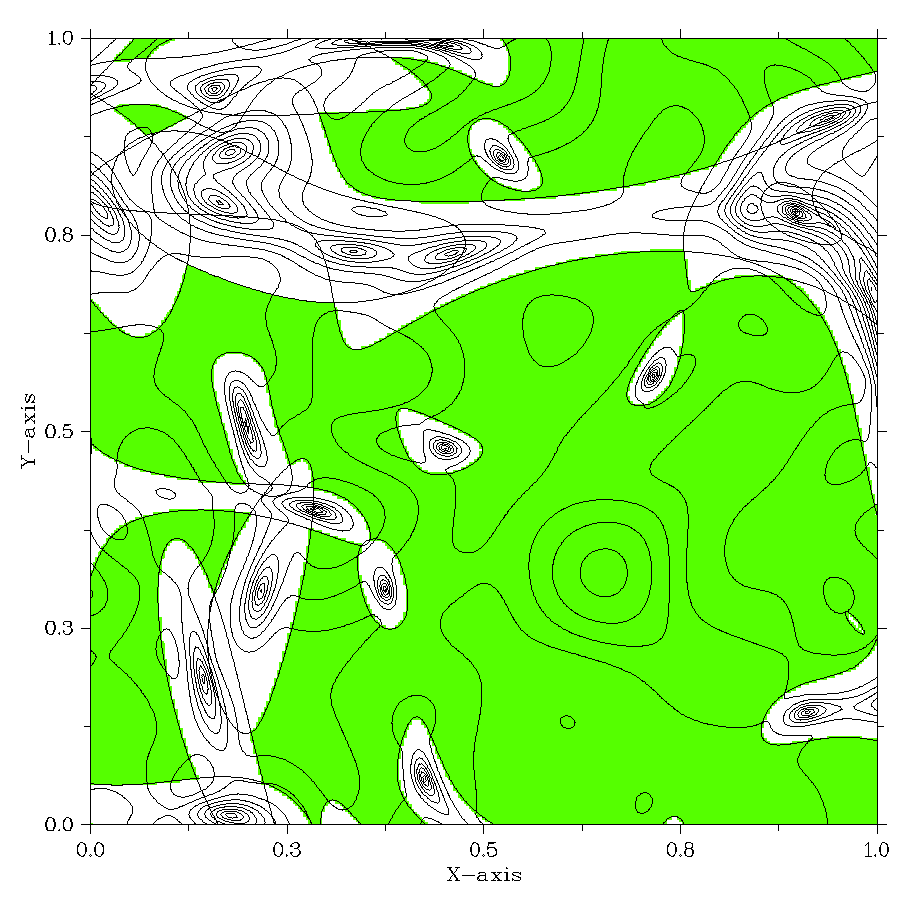
\includegraphics[width=1.0\linewidth]{vag_06.png} \\ (a)}
\end{minipage}
\hfill
\begin{minipage}[h]{0.5\linewidth}
\center{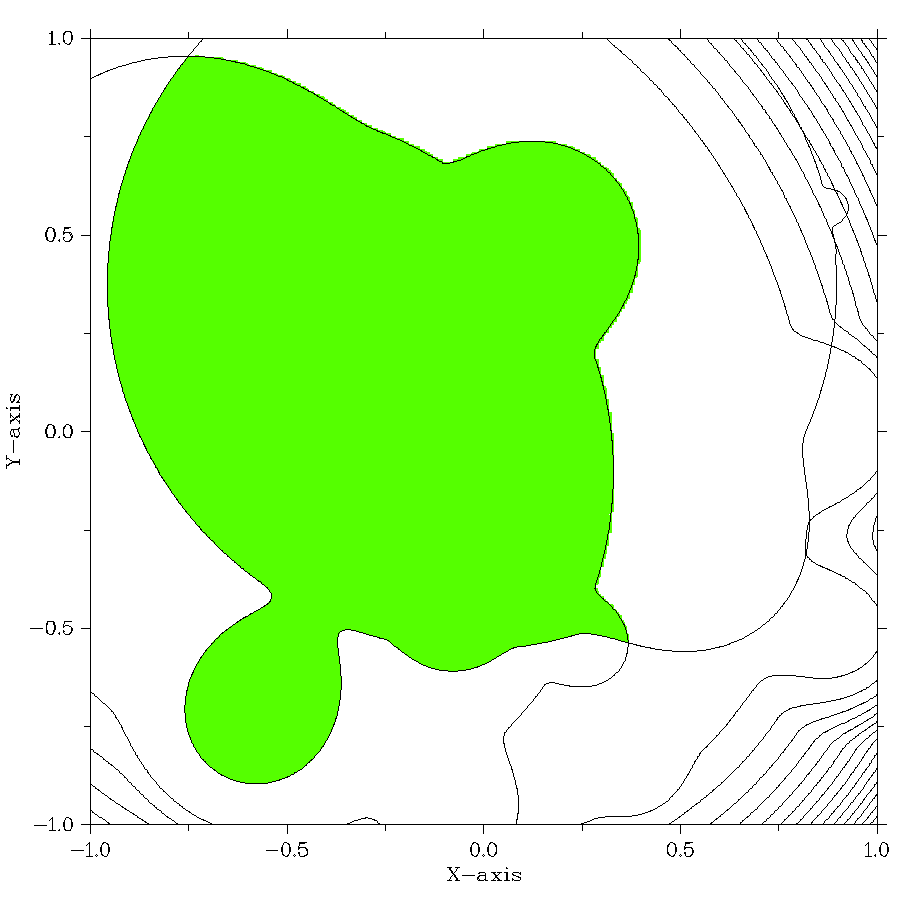
\includegraphics[width=1.0\linewidth]{GKLS_04.png} \\ (b)}
\end{minipage}
\caption{The level lines of (a) hard and (b) simple subproblems}
\label{fig:2}
\end{figure}

The numerical experiments were carried out using two classes of problems 
(\textit{Simple} ans \textit{Hard}) with $N=5$. The problem was considered to 
be solved if the algorithm generates a trial point $y^k$ in $\delta$-vicinity 
of the global minimizer, i.e. $\left\|y^k-y^\ast\right\|\leq\delta$ . The 
size of the vicinity was selected as $\delta=0.01\left\|b-a\right\|$, where 
$a$ and $b$ are the boundaries of the search domain $D$. The maximum 
allowable number of iterations was $K_{max} = 10^6$.

Let us conduct the first experiment by solving the \textit{Simple} and \textit{Hard} problem 
series on a single node employing both available CPUs in full (i.e. $p=16$ 
cores available). In table \ref{tab:1} the averaged time (in seconds) 
required to solve the problems of the series is presented.

\begin{table}
\caption{Average time for solving the problem on one node}
\label{tab:1}
\begin{center}
\begin{tabular}{cc}
\hline
Problems & Time (sec) \\
\hline
\textit{Hard} & 52  \\
\textit{Simple} & 51 \\
\hline
\end{tabular}
\end{center}
\end{table}

Let us conduct the next experiment employing $p$ nodes each including three 
graphic accelerators. Thus, at $p=32$ total 96 GPU accelerators were employed 
each including 2688 CUDA cores; 258048 CUDA cores in all. In tables \ref{tab:2} and \ref{tab:3} the average time and the speedup with respect to the run 
on a single node are presented.

\begin{table}
\caption{Average time for solving the problem on $p$ nodes}
\label{tab:2}
\begin{center}
\begin{tabular}{cccc}
\hline
Problems & $p = 8$ & $p=16$ & $p=32$ \\
\hline
\textit{Hard} & 11.51 & 5.53 & 0.54 \\
\textit{Simple} & 2.04 & 1.50 & 0.47\\
\hline
\end{tabular}
\end{center}
\end{table}

\begin{table}
\caption{Speedup with respect to one node}
\label{tab:3}
\begin{center}
\begin{tabular}{cccc}
\hline
Problems & $p = 8$ & $p=16$ & $p=32$ \\
\hline
\textit{Hard} & 5 & 9 & 96\\
\textit{Simple} & 25 & 34& 109\\
\hline
\end{tabular}
\end{center}
\end{table}

The results of experiments demonstrate that the parallel index algorithm combined with the nested optimization scheme provides a good speedup on the considered problem class. 

%The results of experiments performed on a series of test problems of the constrained global optimization with different time of computing the problem functions demonstrate the index global optimization algorithm combined with the block recursive scheme for the dimensionality reduction to provide a good speedup on the considered problem class. The directions of further investigations include the expansion of the number of algorithms used for solving the subproblems on the GPUs.

\section*{Acknowledgments}
This research was supported by the Russian Science Foundation, project No 16-11-10150 ``Novel efficient methods
and software tools for the time consuming decision making problems with using supercomputers of superior performance''.

\bigskip

\section*{References}

\medskip

\begin{thebibliography}{9}

\bibitem{Strongin2000}
Strongin R G and Sergeyev Ya D 2000 \textit{Global Optimization with Non-Convex Constraints. Sequential 
and Parallel Algorithms} (Dordrecht: Kluwer Academic Publishers)

\bibitem{Strongin2013}
Strongin R G, Gergel V P, Grishagin V A and Barkalov K A 2013  \textit{Parallel Computing in Global Optimization Problems} (Moscow: Moscow State University Press) (in Russian).

\bibitem{Globalizer}
Sysoyev A V, Barkalov K A, Sovrasov V V, Lebedev I G and Gergel V P 2017 \textit{Lect. Notes Comput. Science} \textbf{10421} 492--499

\bibitem{Globalizer1}
Gergel  V, Barkalov K and Sysoyev A 2018 \textit{Numer. Algebra Contr. Optim.} \textbf{8(1)} 47--62

\bibitem{Jones}
Floudas C A and Pardalos P M 2009 \textit{The Encyclopedia of Optimization } (Heidelberg: Springer) p 725--735 

\bibitem{Zilinskas}
Paulavi\v{c}ius R, \v{Z}ilinskas J and Grothey A 2011 \textit{Optim. Meth. Soft.} \textbf{26(3)} 487--498

\bibitem{Evtushenko2009}
Evtushenko Yu G, Malkova V U and Stanevichyus A A 2009 \textit{Comput. Math. Math. Phys.} \textbf{49(2)} 246--260.

\bibitem{Evtushenko2014}
Evtushenko Yu G and Posypkin M A 2014 \textit{Autom. Remote Control} \textbf{75(6)} 1025--1040

\bibitem{Strongin2017}
Barkalov K A and Strongin R G 2017 \textit{Lect. Notes Comput. Science} \textit{10556} 18--33

\bibitem{BarkalovGergelLebedev2016}
Barkalov K, Gergel V and Lebedev I  2016 \textit{AIP Conf. Proc.} \textbf{1738} 400006

\bibitem{BarkalovLebedev}
Barkalov K A and Lebedev I G 2016 \textit{Commun. Comp. Inf. Science} \textbf{687} 224--235

\bibitem{Gergel2005}
Gergel V P and Strongin R G 2003 \textit{Lect. Notes Comput. Science} \textit{2763} 76--88

\bibitem{GergelLebedev}
Gergel V and Lebedev I 2015 \textit{Proc. Comput. Science} \textbf{66} 53--62

\bibitem{GergelSidorov}
Gergel V and Sidorov S 2015 \textit{Lect. Notes Comput. Science} \textbf{9251} 505--515

\bibitem{Gergel2017}
Gergel V 2017 \textit{Lect. Notes Comput. Science} \textbf{10556} 314--319

\bibitem{Gergel2016}
Gergel V, Grishagin V and Gergel A 2016 \textit{J. Glob. Optim.} \textbf{66(1)} 35--51

\bibitem{Sergeyev2015}
Sergeyev Y D and Kvasov D E 2015 \textit{Commun. Nonlinear Sci. Numer. Simul.} \textbf{21(1-3)} 99--111

\end{thebibliography}

\end{document}


